\documentclass[12pt,a4paper,oneside]{report}

% =========================
% Préambule — VisionGuard PFE
% ENISo 2025-2026 — Yahya
% =========================

% Encodage et langue
\usepackage[utf8]{inputenc}
\usepackage[T1]{fontenc}
\usepackage[french]{babel}
\usepackage{lmodern}
\usepackage{csquotes}

% Mise en page
\usepackage{geometry}
\geometry{left=2cm,right=2cm,top=2cm,bottom=2.5cm}
\usepackage{setspace}
\onehalfspacing
\setlength{\headheight}{15.5pt}
\usepackage{parskip}
\setlength{\parindent}{0.7cm}

% Graphiques, tableaux, figures
\usepackage{graphicx}
\graphicspath{{figures/}}
\usepackage{float}
\usepackage{caption}
\captionsetup[figure]{
    font=small,
    labelfont=it,
    textfont=it,
    labelsep=colon,
    name=Figure,
    justification=centering
}
\captionsetup[table]{
    font=small,
    labelfont=it,
    textfont=it,
    labelsep=colon,
    name=Tableau,
    justification=centering
}
\usepackage{subcaption}
\usepackage{array}
\usepackage{longtable}
\usepackage{booktabs}
\usepackage{multirow}
\usepackage{tabularx}
\usepackage{xcolor}
\usepackage{colortbl}
\setlength{\arrayrulewidth}{0.4pt}
\usepackage{tikz}
\usetikzlibrary{arrows.meta,positioning,shapes.geometric,fit}
% Liens et références
\usepackage[hidelinks]{hyperref}
\usepackage{cleveref}

% tocloft
\usepackage{tocloft}

% Code source
\usepackage{listings}
\lstdefinestyle{rapportcode}{
    basicstyle=\ttfamily\small,
    breaklines=true,
    frame=single,
    numbers=left,
    numberstyle=\tiny,
    keywordstyle=\bfseries,
    commentstyle=\itshape,
    showstringspaces=false,
    tabsize=2
}
\lstset{style=rapportcode}

% Bibliographie
\usepackage[backend=biber,style=numeric,sorting=none]{biblatex}
\addbibresource{bibliography.bib}

% Titres chapitres et sections
\usepackage{titlesec}

% Chapitre : bold, large, no underline
\titleformat{\chapter}[block]
  {\normalfont\Large\bfseries}
  {Chapitre \thechapter : }
  {0pt}
  {\Large\bfseries}
\titlespacing*{\chapter}{0pt}{-35pt}{10pt}

% Section : numérotée, bold, same size as body
\titleformat{\section}
  {\normalfont\normalsize\bfseries}
  {\thesection}
  {1.5em}{}

% Sous-section : numérotée, bold
\titleformat{\subsection}
  {\normalfont\normalsize\bfseries}
  {\thesubsection}
  {1.5em}{}

% Sous-sous-section
\titleformat{\subsubsection}
  {\normalfont\normalsize\itshape}
  {\thesubsubsection}
  {1.5em}{}

% En-têtes et pieds de page
\usepackage{fancyhdr}
\pagestyle{fancy}
\fancyhf{}
\fancyhead[L]{\small\nouppercase{\leftmark}}\fancyfoot[C]{\thepage}
\renewcommand{\headrulewidth}{0.4pt}
\fancypagestyle{plain}{\fancyhf{}\fancyfoot[C]{\thepage}\renewcommand{\headrulewidth}{0pt}}
% Commandes utiles
\newcommand{\todo}[1]{\textcolor{red}{\textbf{TODO :} #1}}
\newcommand{\placeholderfigure}[2]{%
\begin{figure}[H]
\centering
\begin{tikzpicture}
\draw[dashed, rounded corners] (0,0) rectangle (12,5);
\node[align=center] at (6,2.5) {\textbf{Image à insérer}\\#1};
\end{tikzpicture}
\caption{#2}
\end{figure}
}

\begin{document}
\assignpagestyle{\chapter}{fancy}
% =========================
% Page de garde
% =========================
\begin{titlepage}
\thispagestyle{empty}
\centering

\noindent
\begin{minipage}{0.4\textwidth}
    \raggedright
    \textbf{Réf :}
\end{minipage}
\hfill
\begin{minipage}{0.4\textwidth}
    \raggedleft
    \textbf{AU : 2025--2026}
\end{minipage}
\vspace{0.001cm}

{\LARGE Université de Sousse}

{\color{cyan!25}\rule{0.90\textwidth}{3.5pt}}

\vspace{0.01cm}

{\LARGE École Nationale d'Ingénieurs de Sousse}

\vspace{0.01cm}


\includegraphics[width=3.8cm]{Logo_ENISo.png}

\vspace{0.1cm}

{\Large Département Génie Mécatronique}

\vspace{0.1cm}

{\large Rapport de Projet de Fin d'Études}

\vspace{0.01cm}

{\normalsize Présenté en vue de l'obtention du } \\
{\large \textbf{Diplôme d'Ingénieur}}

\vspace{0.01cm}

{\color{cyan!25}\rule{0.90\textwidth}{3.5pt}}

\vspace{0.1cm}

\begin{minipage}{0.9\textwidth}
\centering
{\Large \textbf{VisionGuard – Système de Contrôle Qualité Automatisé par Vision Industrielle}}
\end{minipage}

\vspace{0.1cm}

{\color{cyan!25}\rule{0.90\textwidth}{3.5pt}}

\vspace{0.1cm}

{\normalsize Réalisé par : \textbf{Ben Turkia Yahya}}

\vspace{0.1cm}

{\normalsize Organisme d'accueil : \textbf{Pursuit Aerospace Tunisia — Site El Mghira}}

\vspace{0.3cm}

% Placeholder logo entreprise — remplacer par le vrai logo

\includegraphics[width=4.7cm]{pursuit_logo0.png}
\vspace{0.3cm}

{\normalsize \textbf{Soutenu le \hspace{1cm} / \hspace{0.5cm} / 2026 devant le jury :}}

\vspace{0.1cm}

\begin{tabular}{lll}
Président            & : & M. / Mme Nom Prénom, ENISo \\[0.15cm]
Rapporteur           & : & M. / Mme Nom Prénom, ENISo \\[0.15cm]
Encadrant académique & : & M.Saafi Houssem, ENISo              \\[0.15cm]
Encadrant industriel & : & M.Mokni Alaeddine, Pursuit Aerospace \\
\end{tabular}

\vfill

\begin{flushright}
{\normalsize \copyright\ Ben Turkia Yahya 2026}
\end{flushright}

\end{titlepage}

% =========================
% Page des signatures
% =========================
\clearpage
\thispagestyle{empty}

\begin{center}

\vspace*{1.8cm}

{\LARGE \textit{\textbf{Signatures des encadrants}}}

\vspace{2.2cm}

\setlength{\fboxsep}{100pt} % Ajustez la valeur pour augmenter ou réduire l'espace à l'intérieur de la boîte
\fbox{
    \begin{minipage}[c][0cm][c]{0cm}
        \centering
    \end{minipage}
}

\vspace{0.35cm}

{\normalsize M. Ala — Encadrant académique, ENISo}

\vspace{1.0cm}

\fbox{
    \begin{minipage}[c][0cm][c]{0cm}
        \centering
    \end{minipage}
}

\vspace{0.35cm}

{\normalsize M. Houssem — Encadrant industriel, Pursuit Aerospace}

\end{center}

\clearpage

% =========================
% Pages préliminaires
% =========================
\pagenumbering{roman}

\chapter*{Remerciements}
\addcontentsline{toc}{chapter}{Remerciements}

\todo{Rédiger les remerciements ici.}

\chapter*{Résumé}
\addcontentsline{toc}{chapter}{Résumé}

\todo{Rédiger le résumé en français ici. 150--200 mots. Contexte industriel, problématique, solution proposée, résultats obtenus.}

\vspace{1cm}
\noindent\textbf{Mots-clés :} inspection automatisée, vision par ordinateur, noyau céramique, apprentissage profond, contrôle qualité, systèmes embarqués, STM32, Raspberry Pi.

\chapter*{Abstract}
\addcontentsline{toc}{chapter}{Abstract}

\todo{Write the abstract in English here. 150--200 words. Industrial context, problem statement, proposed solution, results.}

\vspace{1cm}
\noindent\textbf{Keywords:} automated inspection, computer vision, ceramic core, deep learning, quality control, embedded systems, STM32, Raspberry Pi.


\tableofcontents
\clearpage
\listoffigures
\clearpage
\listoftables
\clearpage

\chapter*{Liste des Abréviations}
\addcontentsline{toc}{chapter}{Liste des Abréviations}

\begin{tabular}{ll}
\textbf{AI}     & Artificial Intelligence (Intelligence Artificielle) \\
\textbf{CAD}    & Computer-Aided Design \\
\textbf{CNN}    & Convolutional Neural Network \\
\textbf{CSI}    & Camera Serial Interface \\
\textbf{FOV}    & Field of View \\
\textbf{GPIO}   & General Purpose Input/Output \\
\textbf{HAL}    & Hardware Abstraction Layer \\
\textbf{IMX296} & Capteur d'image Sony (RPi HQ Camera) \\
\textbf{NEMA}   & National Electrical Manufacturers Association \\
\textbf{PFE}    & Projet de Fin d'Études \\
\textbf{RPi5}   & Raspberry Pi 5 \\
\textbf{SCP}    & Secure Copy Protocol \\
\textbf{SSH}    & Secure Shell \\
\textbf{STM32}  & Microcontrôleur STMicroelectronics (famille STM32) \\
\textbf{TCP}    & Transmission Control Protocol \\
\textbf{TMC2208}& Driver moteur pas à pas (Trinamic) \\
\textbf{UART}   & Universal Asynchronous Receiver-Transmitter \\
\textbf{USB}    & Universal Serial Bus \\
\end{tabular}


\clearpage
\pagenumbering{arabic}

% =========================
% Corps du rapport
% =========================
\chapter*{Introduction Générale}
\addcontentsline{toc}{chapter}{Introduction Générale}

\todo{Rédiger l'introduction générale ici. 1--1.5 pages. Contexte industriel aérospatial, enjeux qualité, problématique inspection M00, présentation de la solution VisionGuard, plan du rapport.}

\chapter{Contexte industriel et cadre du projet}

\section{Introduction}
Ce premier chapitre vise à introduire le cadre général du projet. La première partie est
consacrée à la présentation de Pursuit Aerospace, à l'échelle mondiale puis à travers son
entité tunisienne, en mettant l'accent sur le site d'El Mghira où le projet a été réalisé.
La deuxième partie présente le contexte des ceramic cores, le mode d'inspection actuel,
ainsi que la pièce M00 étudiée. Enfin, ce chapitre définit la problématique du projet,
les objectifs visés et la démarche de travail adoptée pour aboutir à la conception d'un
système d'inspection automatisé.

\section{Présentation de l'entreprise d'accueil}

\subsection{Pursuit Aerospace dans le monde}
Pursuit Aerospace est un groupe international spécialisé dans la fabrication de composants
complexes de haute précision destinés principalement aux moteurs aéronautiques. L'entreprise
est issue de la fusion entre Whitcraft et Paradigm Precision, donnant naissance à Pursuit
Aerospace en 2023. Le groupe est implanté dans plusieurs pays, notamment les États-Unis,
le Canada, l'Angleterre et la Tunisie, et s'appuie sur des procédés industriels avancés
pour répondre aux exigences du secteur aéronautique.

\begin{figure}[H]
\centering

\includegraphics[width=9cm]{pursuit_logo.png}
\caption{Logo de Pursuit Aerospace.}
\label{fig:pursuit_logo}
\end{figure}

\subsection{Pursuit Aerospace Tunisia}
Pursuit Aerospace Tunisia a été officiellement créée le 19 septembre 2000, sous forme
de société anonyme (S.A). Elle dispose de deux sites industriels : le premier est situé
à Mégrine, sur la route de Sousse (GP1 KM7, Mégrine 2033), et le second dans la zone
industrielle Mghira 3, Fouchana 2082. Le présent projet a été réalisé au sein de ce
second site.

En 2023, le capital social de l'entreprise s'élève à 2~300~000 dinars tunisiens. Elle
est placée sous la direction de M. Adel Saoudi, Directeur Général, et emploie un
effectif de 530 personnes, réparties selon les tranches d'âge présentées dans la
figure ci-dessous. L'entreprise occupe une superficie totale de 13~800~m², dont
9~600~m² de surface de production couverte.

\begin{figure}[H]
\centering
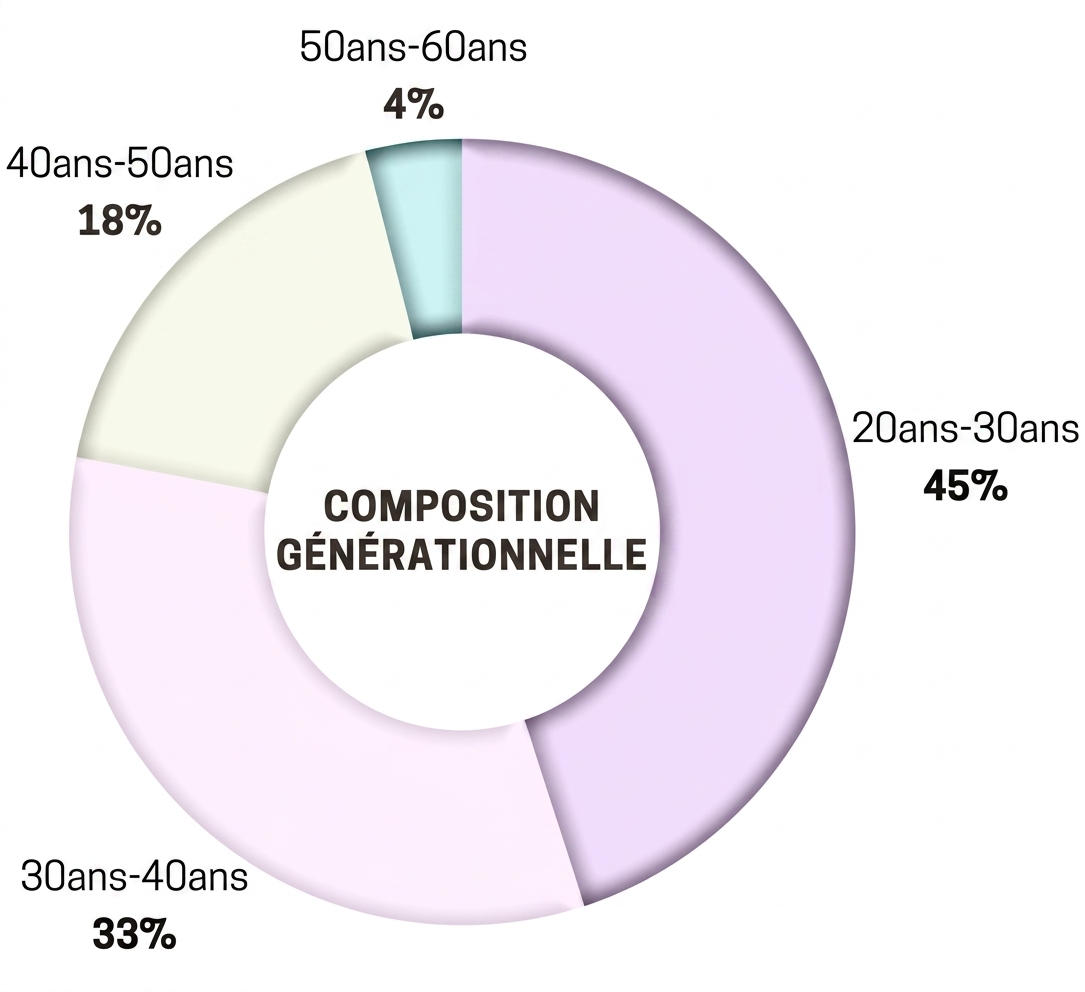
\includegraphics[width=6cm]{generational_makeup.png}
\caption{Répartition par tranches d'âge des effectifs de Pursuit Aerospace Tunisia.}
\label{fig:effectifs}
\end{figure}

\subsection{Produits et familles de produits}
Pursuit Aerospace Tunisia fabrique différentes familles de composants aéronautiques
complexes, principalement destinés aux moteurs. Parmi les familles produites, on retrouve
notamment les swirlers, mixers, cyclones, flanges, plates, elbows, connectors, structural
airfoils, shrouds et flow path components. Ces pièces sont généralement réalisées à partir
d'alliages techniques à base de cobalt ou de nickel et sont associées à plusieurs programmes
moteurs majeurs.

\begin{figure}[H]
\centering
\includegraphics[width=12cm]{/home/yahya/Pictures/Screenshots/Exemples de pièces produites chez Pursuit Aerospace Tunisia.png}
\caption{Exemples de pièces produites chez Pursuit Aerospace Tunisia.}
\label{fig:pieces_pursuit}
\end{figure}

\subsection{Clients et exigences qualité}
Pursuit Aerospace travaille avec des clients majeurs du secteur aéronautique et énergétique.
Parmi les clients figurent notamment GE Aviation, Safran, Rolls-Royce, Woodward, Avio Aero
et Unison. Ces clients imposent des exigences strictes en matière de qualité, de précision,
de traçabilité et de stabilité du processus de fabrication. Dans ce contexte, la maîtrise
du contrôle qualité représente un élément essentiel pour garantir la conformité des produits.

\begin{figure}[H]
\centering

\includegraphics[width=12cm]{clients_pursuit.png}
\caption{Principaux clients de Pursuit Aerospace.}
\label{fig:clients}
\end{figure}

\subsection{Certifications et système qualité}
La qualité constitue un axe central dans l'activité de Pursuit Aerospace. L'entreprise
dispose de certifications telles que AS9100 et ISO 9001, ainsi que d'accréditations NADCAP
pour certains procédés industriels spécifiques. Ces certifications traduisent l'engagement
de l'entreprise envers la conformité, l'amélioration continue et la satisfaction client.

\subsection{Organisation générale}
L'organisation de Pursuit Aerospace Tunisia regroupe plusieurs fonctions industrielles et
supports, notamment la production, la qualité, les méthodes, la maintenance, l'ingénierie
et les ressources humaines. Cette organisation permet d'assurer la coordination entre les
différentes activités nécessaires à la fabrication et au contrôle des composants
aéronautiques. Le présent projet s'inscrit dans cet environnement industriel, plus
précisément au niveau du site El Mghira et de l'inspection visuelle des ceramic cores.

\begin{figure}[H]
\centering
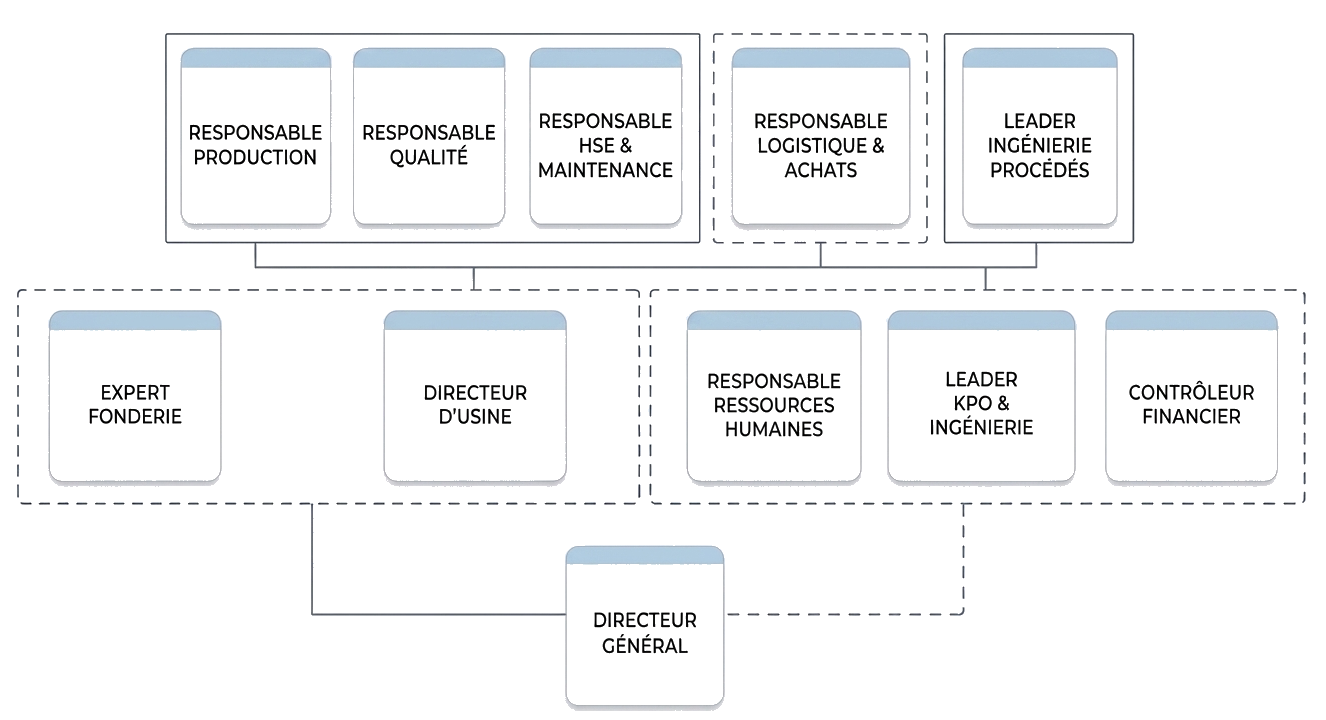
\includegraphics[width=12cm]{organigramme_pursuit.png}
\caption{Organigramme de Pursuit Aerospace Tunisia.}
\label{fig:organigramme}
\end{figure}

\section{Les ceramic cores chez Pursuit Aerospace}

\subsection{Rôle dans le procédé de fabrication et utilisation au site El Mghira}
Dans le procédé de fonderie à la cire perdue pratiqué chez Pursuit Aerospace, les ceramic
cores jouent un rôle indispensable. Ils permettent de former les cavités internes complexes
des composants métalliques coulés, notamment les géométries en veine qui ne peuvent pas
être obtenues par usinage après coulée. Le ceramic core est intégré dans le modèle en cire
avant l'opération de moulage, puis éliminé après solidification du métal afin de libérer
les cavités internes de la pièce finale.



Au site El Mghira, une activité dédiée aux ceramic cores a été développée. Elle regroupe
plusieurs opérations telles que la préparation de la matière céramique, l'injection, le
frittage, le nettoyage et l'imprégnation. Ces étapes permettent d'obtenir des cores
suffisamment précis et résistants pour être utilisés dans le procédé de fonderie à la
cire perdue.

\begin{figure}[H]
\centering
\todo{Insérer figure : vue générale de l'unité ceramic cores au site El Mghira.}
\caption{Vue générale de l'unité ceramic cores au site El Mghira.}
\label{fig:unite_ceramic}
\end{figure}

\subsection{Inspection actuelle des ceramic cores : principe, moyens et limites}
L'inspection actuelle des ceramic cores au site El Mghira repose principalement sur un
contrôle visuel manuel. L'opérateur manipule les pièces une par une et observe les surfaces
accessibles afin d'identifier d'éventuels défauts visibles tels que les pores, les fissures,
les piqûres ou les zones de matière manquante.

\begin{figure}[H]
\centering
\todo{Insérer figure : poste d'inspection visuelle manuelle actuel.}
\caption{Poste d'inspection visuelle manuelle actuel au site El Mghira.}
\label{fig:poste_inspection}
\end{figure}

Pour les cores présentant des veines internes, l'inspection nécessite une observation plus
attentive. La pièce est orientée progressivement par l'opérateur à l'aide d'un support
rotatif manuel. L'observation des veines est réalisée avec l'aide d'un éclairage local et
d'un support optique ou d'une lentille, afin de mieux visualiser les surfaces internes.

\begin{figure}[H]
\centering
\todo{Insérer figure : support rotatif manuel avec éclairage et support optique.}
\caption{Support rotatif manuel avec éclairage utilisé pour l'inspection des veines.}
\label{fig:support_rotatif}
\end{figure}

Cette approche présente plusieurs limites importantes. Premièrement, la détection de défauts
de petite taille --- notamment des pores inférieurs au millimètre situés sur les parois
internes des veines --- dépend fortement de la vigilance et de l'expérience de l'opérateur,
introduisant une variabilité humaine significative. Deuxièmement, l'accès optique aux
surfaces internes des veines en chevron est géométriquement difficile en raison de leur
orientation angulaire et de l'étroitesse de l'ouverture. Troisièmement, avec 40 veines et
deux parois par veine, le nombre total de surfaces à inspecter est de 80, rendant un
contrôle manuel exhaustif impossible à garantir dans des délais industriels acceptables.

\section{La pièce M00 : géométrie et surfaces critiques}

\subsection{Description générale et géométrie des veines internes}
Dans le cadre de son activité, Pursuit Aerospace Tunisia intègre des ceramic cores dans son procédé 
de fonderie à la cire perdue afin de former les cavités internes complexes des composants 
métalliques coulés des géométries qui ne peuvent être obtenues par usinage après coulée. 
Au site El Mghira plus particulièrement, une activité dédiée à la production de ces cores a été développée, 
couvrant l'ensemble des opérations de transformation : injection, frittage, nettoyage et imprégnation, 
pour obtenir des pièces céramiques précises et mécaniquement résistantes.
\begin{figure}[H]
\centering
\todo{Insérer figure : vue d'ensemble des différentes références de ceramic cores.}
\caption{Vue d'ensemble des différentes références de ceramic cores produits sur le site.}
\label{fig:refs_cores}
\end{figure}

La pièce M00 est un disque annulaire monolithique en céramique, de couleur rose mat et
de surface non réfléchissante. Ses dimensions principales sont les suivantes : diamètre
extérieur d'environ 84,74~mm, diamètre intérieur d'environ 43,52~mm, et hauteur de
23,3~mm.

\begin{figure}[H]
\centering
\todo{Insérer figure : vues CAO de la pièce M00 (face, profil, perspective).}
\caption{Vues CAO de la pièce M00 : face, profil et perspective.}
\label{fig:cao_m00}
\end{figure}

La particularité géométrique de cette pièce réside dans la présence de 40 veines
traversantes régulièrement réparties sur la circonférence, de forme en chevron. Ces
veines constituent les éléments fonctionnels du core : elles forment, après coulée et
lixiviation, les canaux internes de la pièce métallique finale. Chaque veine présente
deux parois latérales internes --- une paroi gauche et une paroi droite --- dont l'état
de surface conditionne directement la qualité du composant produit.

\begin{figure}[H]
\centering
\todo{Insérer figure : zoom sur la géométrie d'une veine en chevron.}
\caption{Zoom sur la géométrie d'une veine en chevron de la pièce M00.}
\label{fig:veine_chevron}
\end{figure}

\subsection{Défauts ciblés, taille minimale et difficultés de détection}
Les défauts recherchés sur la pièce M00 sont principalement des pores et des piqûres
localisés sur les parois internes des veines, pouvant apparaître au cours du procédé de
fabrication du core. La taille minimale de défaut à détecter est fixée à 0,8~mm de
diamètre. Ces défauts, s'ils ne sont pas détectés à temps, peuvent affecter la conformité
du core et influencer la qualité du procédé de fabrication associé.

\begin{figure}[H]
\centering
\todo{Insérer figure : exemples de défauts (pores/piqûres) sur paroi interne de veine.}
\caption{Exemples de défauts de type pores et piqûres sur paroi interne de veine.}
\label{fig:defauts_m00}
\end{figure}

La détection de ces défauts présente plusieurs difficultés : la surface céramique matte
et de couleur uniforme offre peu de contraste naturel, l'orientation angulaire des veines
limite l'accès optique direct, et le nombre élevé de surfaces à couvrir rend le contrôle
manuel non exhaustif et non reproductible.

\section{Problématique, objectifs et méthodologie adoptée}

\subsection*{Problématique}
L'inspection manuelle des ceramic cores M00, telle qu'elle est pratiquée actuellement,
présente des limites pour garantir une détection fiable et exhaustive des défauts
surfaciques situés sur les parois internes des veines. En raison de la géométrie complexe
de la pièce, de l'accès visuel difficile aux zones internes et du nombre élevé de surfaces
à contrôler, le développement d'une solution d'inspection automatisée, reproductible et
documentable devient nécessaire afin de fiabiliser le contrôle et de mieux répondre aux
exigences de qualité du contexte aéronautique.

\subsection*{Objectifs}
L'objectif général de ce projet est de concevoir et développer un système d'inspection
automatisé dédié au contrôle des ceramic cores M00, capable de détecter des défauts de
type pore ou piqûre d'un diamètre minimal de 0,8~mm sur les 80 surfaces internes des
veines, avec un temps de cycle inférieur ou égal à 3 minutes par pièce.

Les objectifs spécifiques sont :
\begin{itemize}
    \item Concevoir un système mécanique permettant l'indexation de la pièce et le
    positionnement de la caméra face à chaque veine ;
    \item Mettre en place une chaîne d'acquisition d'images adaptée à la géométrie et
    aux caractéristiques optiques de la pièce ;
    \item Développer et intégrer un module de classification par intelligence artificielle
    permettant de distinguer les surfaces conformes des surfaces présentant des défauts
    visibles ;
    \item Valider le concept par un prototype fonctionnel et une preuve de concept du
    module IA.
\end{itemize}

\subsection*{Démarche de travail}
La démarche adoptée suit une progression en cinq phases : formalisation du besoin et
structuration des exigences, conception mécanique, optique, électronique et logicielle
du système, développement et intégration du module IA, réalisation physique du prototype,
puis tests et validation.

\begin{figure}[H]
\centering
\todo{Insérer figure : diagramme de Gantt du projet (mai-juin 2026).}
\caption{Diagramme de Gantt du projet VisionGuard.}
\label{fig:gantt}
\end{figure}

\section{Conclusion}
Ce chapitre a présenté le cadre industriel du projet : l'entreprise Pursuit Aerospace,
son site El Mghira, le procédé de fabrication des ceramic cores et les limites de
l'inspection manuelle actuelle. La pièce M00 a été identifiée comme objet d'étude en
raison de sa géométrie complexe et du défi d'inspection qu'elle représente. La
problématique et les objectifs du projet ont été formalisés. Le chapitre suivant
présentera la formalisation du besoin selon une approche d'ingénierie système légère,
à travers la délimitation du système, l'identification des cas d'utilisation et la
structuration des exigences fonctionnelles et techniques.
% ============================================================
% Chapitre 2 — Analyse des besoins et spécification des exigences
% VisionGuard PFE — ENISo 2025-2026 — Yahya Ben Turkia
% ============================================================

\chapter{Analyse des besoins et spécification des exigences}

% --------------------------------------------------------
\section{Introduction}
% --------------------------------------------------------

Ce chapitre a pour objectif de formaliser le besoin industriel identifié au chapitre
précédent selon une approche d'ingénierie système légère. Cette démarche vise à délimiter
le système à concevoir, à identifier les acteurs qui interagissent avec lui et à structurer
les exigences fonctionnelles et techniques qui guideront les choix de conception.

Dans un premier temps, le système est situé par rapport à son environnement à travers un
diagramme de contexte et l'identification de ses principales interactions externes. Les cas
d'utilisation sont ensuite présentés afin de décrire les scénarios d'interaction entre les
acteurs et le système. Les exigences sont enfin formalisées dans des tableaux structurés,
destinés à servir de référence pour la conception, la réalisation et la validation du
prototype. Le chapitre se termine par une analyse préliminaire des risques liés à la
conception, à l'intégration et à la validation du système.

% --------------------------------------------------------
\section{Délimitation du système et analyse des interactions}
% --------------------------------------------------------

\subsection{Diagramme de contexte}

Le diagramme de contexte permet de délimiter les frontières du système d'inspection
automatisé VisionGuard par rapport à son environnement extérieur. Il met en évidence les
acteurs externes qui interagissent directement avec le système, ainsi que les principaux
flux physiques, informationnels et énergétiques échangés en conditions réelles
d'utilisation.

Dans ce projet, le système VisionGuard est considéré comme un dispositif d'inspection
semi-automatisé destiné au contrôle des pièces M00. Il reçoit une pièce positionnée par
l'opérateur, réalise l'acquisition des surfaces internes à inspecter, traite les images
acquises et fournit un résultat d'inspection exploitable par l'opérateur et le service
qualité.

Les acteurs externes identifiés sont les suivants :

\begin{itemize}
    \item \textbf{Opérateur} : positionne la pièce M00 sur le support, lance le cycle
    d'inspection et consulte les résultats.
    \item \textbf{Service qualité} : définit les critères d'acceptation et exploite les
    résultats d'inspection pour le suivi de conformité.
    \item \textbf{Pièce M00} : objet physique soumis à l'inspection.
    \item \textbf{Alimentation électrique} : fournit l'énergie nécessaire au fonctionnement
    des sous-systèmes.
    \item \textbf{Environnement atelier} : impose des contraintes d'encombrement, de
    poussière, de manipulation et de robustesse.
    \item \textbf{Maintenance} : impose l'accessibilité aux composants, la facilité de
    réglage et l'entretien du système.
\end{itemize}

\begin{figure}[H]
    \centering
    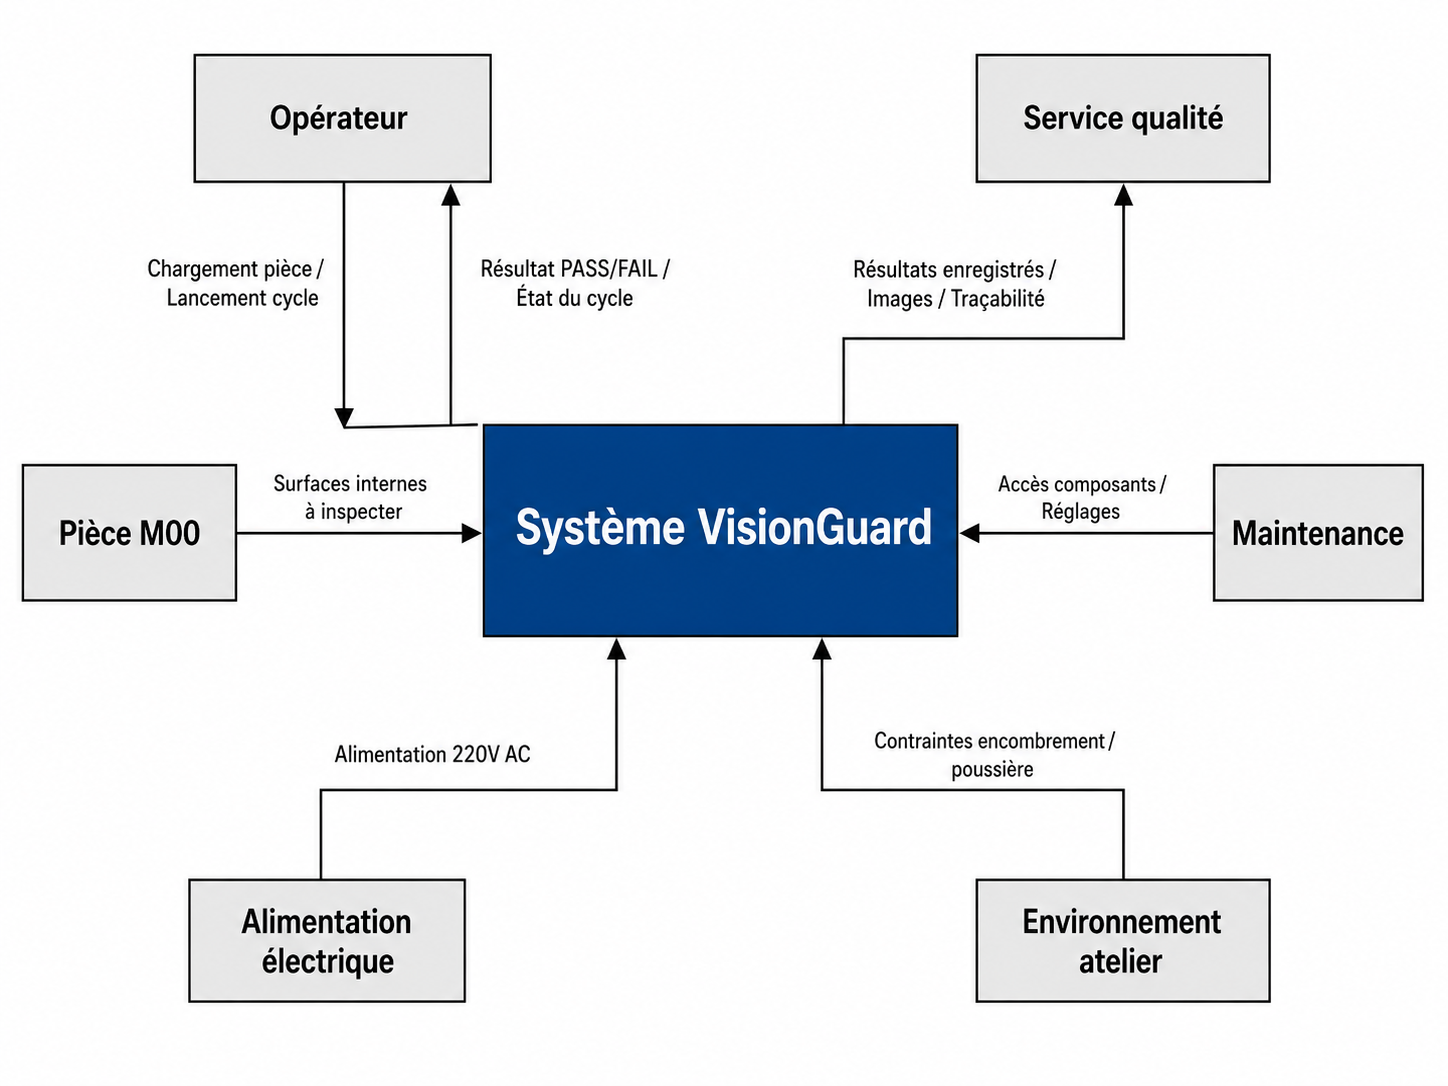
\includegraphics[width=0.85\textwidth]{contexte_visionguard.png}
    \caption{Diagramme de contexte du système VisionGuard.}
    \label{fig:contexte}
\end{figure}

% --------------------------------------------------------
\subsection{Analyse des interactions système-environnement}
\label{sec:interactions}

À partir du diagramme de contexte, les principales interactions entre VisionGuard et son
environnement peuvent être précisées. Cette analyse permet de transformer les échanges
identifiés en exigences fonctionnelles, techniques ou contraintes de conception. Elle
constitue ainsi une étape intermédiaire entre la délimitation du système et la formulation
du cahier des charges.

Le tableau suivant synthétise les interactions retenues.

\renewcommand{\arraystretch}{1.3}
\begin{longtable}{|p{1.5cm}|p{6cm}|p{4cm}|p{4cm}|}
\caption{Interactions entre le système VisionGuard et son environnement.}
\label{tab:interactions} \\
\hline
\rowcolor{gray!20}
\textbf{ID} & \textbf{Interaction} & \textbf{Acteur externe} & \textbf{Nature de l'échange} \\
\hline
\endfirsthead
\hline
\rowcolor{gray!20}
\textbf{ID} & \textbf{Interaction} & \textbf{Acteur externe} & \textbf{Nature de l'échange} \\
\hline
\endhead
\hline
\endfoot
\textbf{I-01} & Chargement et positionnement de la pièce M00 & Opérateur & Entrée physique \\ \hline
\textbf{I-02} & Lancement du cycle d'inspection & Opérateur & Commande utilisateur \\ \hline
\textbf{I-03} & Consultation du résultat d'inspection & Opérateur & Sortie informationnelle \\ \hline
\textbf{I-04} & Exploitation des résultats et images enregistrées & Service qualité & Sortie données / traçabilité \\ \hline
\textbf{I-05} & Présentation des surfaces internes à inspecter & Pièce M00 & Entrée physique \\ \hline
\textbf{I-06} & Alimentation du système & Alimentation électrique & Entrée énergétique \\ \hline
\textbf{I-07} & Contraintes d'encombrement, de poussière et de manipulation & Environnement atelier & Contrainte d'intégration \\ \hline
\textbf{I-08} & Accès aux composants, réglages et opérations d'entretien & Maintenance & Contrainte de maintenabilité \\ \hline
\end{longtable}

% --------------------------------------------------------
\section{Cas d'utilisation}
% --------------------------------------------------------

\subsection{Identification des acteurs}

Dans le cadre du système VisionGuard, deux acteurs principaux interagissent avec le système
lors de son utilisation opérationnelle.

L'opérateur constitue l'acteur principal. Il assure le chargement de la pièce, le lancement
du cycle d'inspection et la consultation du résultat final. Son intervention est limitée aux
actions de préparation, de commande et de supervision~; il n'intervient pas dans le
déroulement automatique de la séquence d'acquisition.

Le service qualité constitue un acteur secondaire. Il exploite les résultats d'inspection
enregistrés à des fins de suivi de conformité, d'analyse des défauts et de traçabilité. Son
interaction avec le système est principalement différée, après la réalisation du cycle
d'inspection.

La maintenance est considérée comme un acteur de contexte. Elle n'intervient pas dans le
cycle nominal d'inspection, mais impose des contraintes de conception relatives à
l'accessibilité, au réglage, au diagnostic et au remplacement des composants.

% --------------------------------------------------------
\subsection{Diagramme de cas d'utilisation}
\label{sec:usecase}

Le diagramme de cas d'utilisation représente les interactions fonctionnelles entre les
acteurs identifiés et le système VisionGuard. Il décrit les scénarios d'utilisation du
système sans préjuger des choix techniques de réalisation.

\begin{figure}[H]
    \centering
    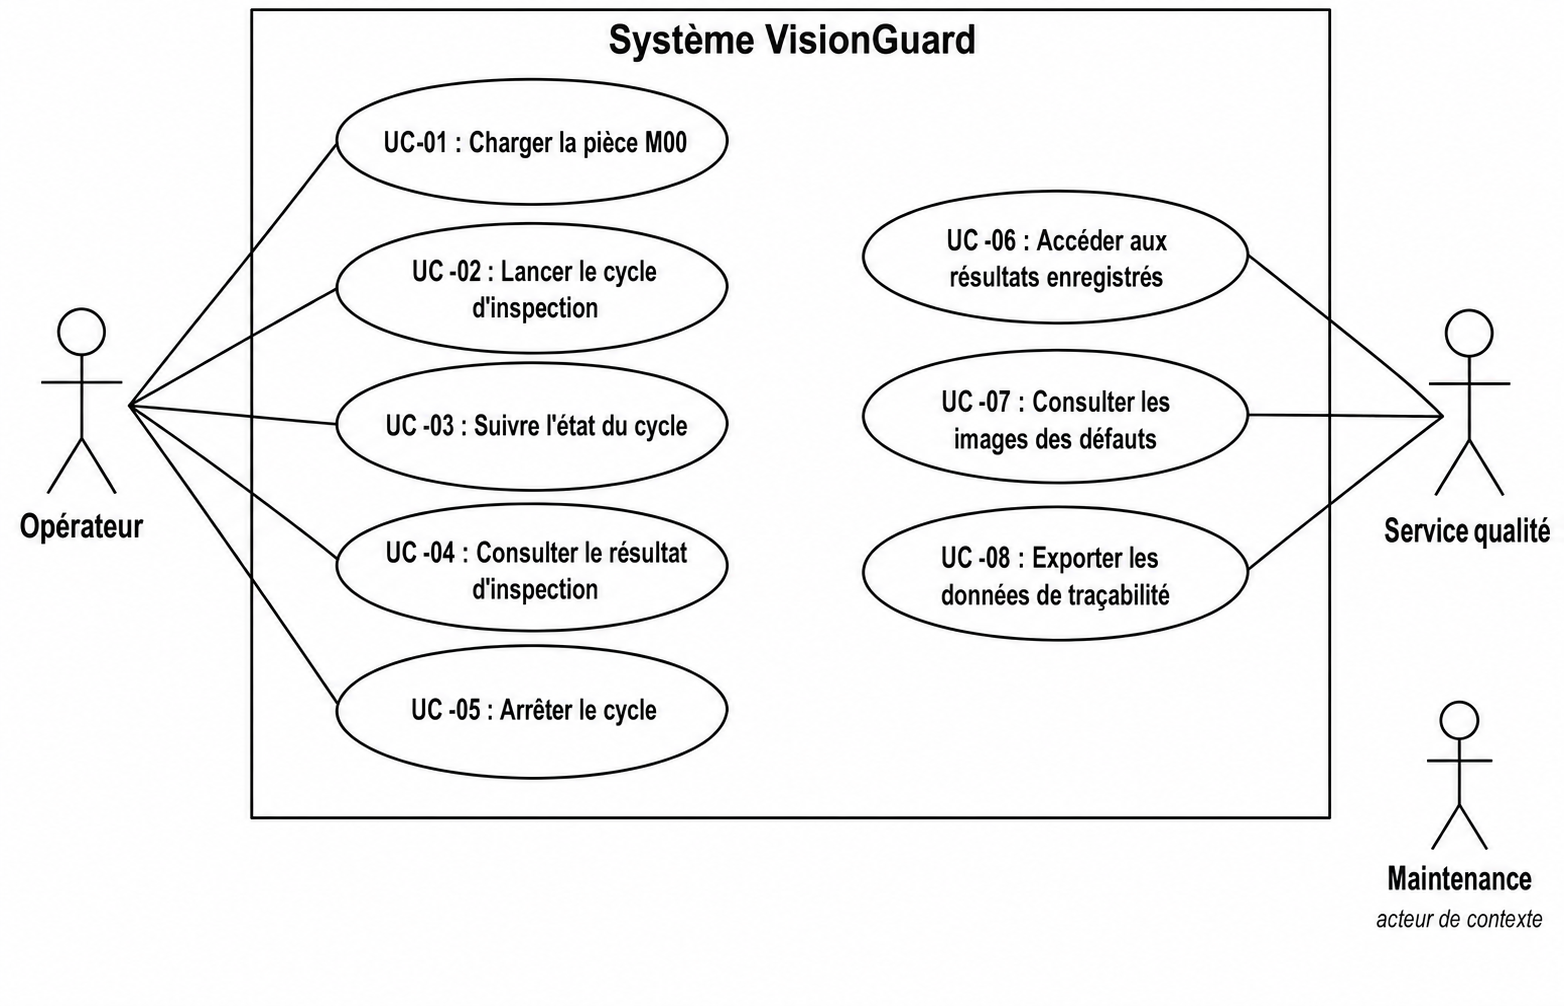
\includegraphics[width=0.90\textwidth]{usecase_visionguard.png}
    \caption{Diagramme de cas d'utilisation du système VisionGuard.}
    \label{fig:usecase}
\end{figure}

% --------------------------------------------------------
\subsection{Description synthétique des cas d'utilisation}

Le tableau suivant présente une description synthétique de chaque cas d'utilisation
identifié, en précisant l'acteur concerné, le scénario nominal et le résultat attendu.

\renewcommand{\arraystretch}{1.3}
\small
\begin{longtable}{|p{1.5cm}|p{2.5cm}|p{5.5cm}|p{4cm}|}
\caption{Description synthétique des cas d'utilisation du système VisionGuard.}
\label{tab:usecase} \\
\hline
\rowcolor{gray!20}
\textbf{ID} & \textbf{Acteur} & \textbf{Scénario nominal} & \textbf{Résultat attendu} \\
\hline
\endfirsthead
\hline
\rowcolor{gray!20}
\textbf{ID} & \textbf{Acteur} & \textbf{Scénario nominal} & \textbf{Résultat attendu} \\
\hline
\endhead
\hline
\endfoot
\textbf{UC-01} & Opérateur
    & L'opérateur place la pièce M00 sur le support rotatif et vérifie son positionnement initial.
    & Pièce prête à être inspectée \\ \hline
\textbf{UC-02} & Opérateur
    & L'opérateur lance le cycle via l'interface utilisateur.
    & Le système démarre la séquence d'inspection. \\ \hline
\textbf{UC-03} & Opérateur
    & L'interface affiche l'état d'avancement de l'inspection en temps réel.
    & L'opérateur est informé de la progression du cycle. \\ \hline
\textbf{UC-04} & Opérateur
    & Le système affiche le résultat global PASS/FAIL et localise les zones défectueuses.
    & L'opérateur dispose du résultat d'inspection. \\ \hline
\textbf{UC-05} & Opérateur
    & L'opérateur interrompt le cycle en cours via l'interface.
    & Le système s'arrête proprement et conserve les données disponibles. \\ \hline
\textbf{UC-06} & Service qualité
    & Le service qualité consulte l'historique des inspections enregistrées.
    & Résultats disponibles avec horodatage et identifiant pièce. \\ \hline
\textbf{UC-07} & Service qualité
    & Le service qualité accède aux images associées aux défauts détectés.
    & Images disponibles pour analyse et décision. \\ \hline
\textbf{UC-08} & Service qualité
    & Le service qualité exporte les données d'inspection.
    & Un fichier de traçabilité est généré. \\ \hline
\end{longtable}

% --------------------------------------------------------
\section{Spécification des exigences}
% --------------------------------------------------------

\subsection{Exigences fonctionnelles}

Les exigences fonctionnelles décrivent ce que le système VisionGuard doit être capable de
réaliser. Elles sont directement dérivées des cas d'utilisation identifiés en
section~\ref{sec:usecase} et des interactions système-environnement définies en
section~\ref{sec:interactions}.

\renewcommand{\arraystretch}{1.3}
\begin{longtable}{|p{1.5cm}|p{10.5cm}|p{2.5cm}|}
\caption{Exigences fonctionnelles du système VisionGuard.}
\label{tab:ef} \\
\hline
\rowcolor{gray!20}
\textbf{ID} & \textbf{Exigence fonctionnelle} & \textbf{Source} \\
\hline
\endfirsthead
\hline
\rowcolor{gray!20}
\textbf{ID} & \textbf{Exigence fonctionnelle} & \textbf{Source} \\
\hline
\endhead
\hline
\endfoot
\textbf{EF-01} & Le système doit permettre le positionnement et l'indexation angulaire de la pièce M00 face aux veines à inspecter.
    & UC-01, I-01 \\ \hline
\textbf{EF-02} & Le système doit acquérir des images exploitables des parois internes des veines.
    & UC-02, I-05 \\ \hline
\textbf{EF-03} & Le système doit permettre l'observation des deux parois internes de chaque veine, soit par orientation contrôlée de la caméra, soit par réglage angulaire validé lors de la phase prototype.
    & UC-02, I-05 \\ \hline
\textbf{EF-04} & Le système doit permettre la détection automatique des défauts de type pore ou piqûre d'un diamètre minimal visé de 0,8~mm.
    & UC-02, I-05 \\ \hline
\textbf{EF-05} & Le système doit afficher un résultat global PASS/FAIL à l'issue de chaque cycle d'inspection.
    & UC-04 \\ \hline
\textbf{EF-06} & Le système doit localiser les veines ou zones présentant des défauts détectés.
    & UC-04, UC-07 \\ \hline
\textbf{EF-07} & Le système doit enregistrer les images acquises avec horodatage et identifiant pièce.
    & UC-06, I-04 \\ \hline
\textbf{EF-08} & Le système doit permettre l'export des données de traçabilité.
    & UC-08 \\ \hline
\textbf{EF-09} & Le système doit permettre l'arrêt propre du cycle en cours de fonctionnement.
    & UC-05 \\ \hline
\end{longtable}

% --------------------------------------------------------
\subsection{Exigences non fonctionnelles}

Les exigences non fonctionnelles définissent les contraintes de performance, d'intégration,
de robustesse et d'environnement auxquelles le système VisionGuard doit se conformer,
indépendamment des fonctions qu'il assure.

\renewcommand{\arraystretch}{1.3}
\small
\begin{longtable}{|p{1.5cm}|p{3cm}|p{3cm}|p{3.5cm}|p{2.5cm}|}
\caption{Exigences non fonctionnelles du système VisionGuard.}
\label{tab:en} \\
\hline
\rowcolor{gray!20}
\textbf{ID} & \textbf{Exigence} & \textbf{Critère de mesure} & \textbf{Niveau exigé} & \textbf{Source} \\
\hline
\endfirsthead
\hline
\rowcolor{gray!20}
\textbf{ID} & \textbf{Exigence} & \textbf{Critère de mesure} & \textbf{Niveau exigé} & \textbf{Source} \\
\hline
\endhead
\hline
\endfoot
\textbf{EN-01} & Temps de cycle d'inspection complet
    & Durée mesurée par pièce
    & $\leq$ 3 minutes
    & Objectif projet \\ \hline
\textbf{EN-02} & Répétabilité de l'indexation angulaire
    & Écart angulaire mesuré sur indexations répétées
    & Écart inférieur à $\pm$1° sur l'ensemble des positions
    & Besoin d'acquisition \\ \hline
\textbf{EN-03} & Résolution spatiale de détection
    & Taille minimale du défaut détectable
    & Défaut visé $\geq$ 0,8~mm de diamètre
    & Besoin qualité \\ \hline
\textbf{EN-04} & Encombrement du système
    & Surface au sol occupée
    & $\leq$ 1~m²
    & Contrainte atelier \\ \hline
\textbf{EN-05} & Alimentation électrique
    & Type de source utilisée
    & 220~V AC secteur standard avec conversions adaptées
    & Contrainte d'intégration \\ \hline
\textbf{EN-06} & Résistance à l'environnement atelier
    & Fonctionnement en présence de poussière céramique et de manipulations répétées
    & Composants protégés et montage robuste
    & Environnement atelier \\ \hline
\textbf{EN-07} & Maintenabilité
    & Accessibilité aux composants et aux réglages
    & Accès possible sans outillage spécifique lourd
    & Maintenance \\ \hline
\textbf{EN-08} & Stabilité mécanique pendant acquisition
    & Netteté des images après indexation
    & Image exploitable sans flou significatif pour la détection du défaut minimal visé
    & Besoin vision \\ \hline
\textbf{EN-09} & Fiabilité de communication entre modules
    & Continuité des échanges pendant un cycle complet
    & Aucune interruption ni commande non exécutée observée lors des tests
    & Besoin d'intégration \\ \hline
\textbf{EN-10} & Sécurité opérateur
    & Protection contre les éléments en mouvement et les risques électriques
    & Respect des pratiques de sécurité en atelier
    & Contrainte sécurité \\ \hline
\end{longtable}

% --------------------------------------------------------
\subsection{Critères de validation associés}

Les critères de validation permettent de vérifier, lors de la phase de tests, que les
exigences formulées sont effectivement satisfaites par le système réalisé. Ils constituent
le lien direct entre la spécification des exigences et les résultats de validation qui
seront présentés au chapitre~5.

\renewcommand{\arraystretch}{1.3}
\small
\begin{longtable}{|p{1.5cm}|p{7cm}|p{7cm}|}
\caption{Critères de validation associés aux exigences.}
\label{tab:validation} \\
\hline
\rowcolor{gray!20}
\textbf{ID} & \textbf{Critère de validation} & \textbf{Méthode de vérification} \\
\hline
\endfirsthead
\hline
\rowcolor{gray!20}
\textbf{ID} & \textbf{Critère de validation} & \textbf{Méthode de vérification} \\
\hline
\endhead
\hline
\endfoot
\textbf{EF-01} & Indexation correcte sur les positions correspondant aux veines
    & Mesure ou observation répétée de l'alignement sur plusieurs cycles \\ \hline
\textbf{EF-02} & Images nettes et exploitables des surfaces inspectées
    & Inspection visuelle des images acquises et contrôle de la netteté \\ \hline
\textbf{EF-03} & Couverture des deux parois internes de chaque veine
    & Vérification de la couverture optique sur une pièce complète ou sur un échantillon représentatif \\ \hline
\textbf{EF-04} & Détection de défauts de référence de taille compatible avec le seuil visé
    & Tests sur pièces non conformes connues ou défauts de référence disponibles \\ \hline
\textbf{EF-05} & Affichage du résultat PASS/FAIL en fin de cycle
    & Test fonctionnel sur pièce conforme et pièce non conforme \\ \hline
\textbf{EF-06} & Localisation correcte des veines ou zones défectueuses
    & Comparaison entre résultat système et inspection manuelle experte \\ \hline
\textbf{EF-07} & Enregistrement des images avec horodatage et identifiant pièce
    & Vérification des fichiers générés après cycle \\ \hline
\textbf{EF-08} & Export fonctionnel des données de traçabilité
    & Test d'export et vérification du contenu du fichier généré \\ \hline
\textbf{EF-09} & Arrêt propre sans perte des données déjà acquises
    & Test d'interruption en cours de cycle \\ \hline
\textbf{EN-01} & Temps de cycle mesuré inférieur ou égal à 3 minutes
    & Chronométrage sur plusieurs cycles d'inspection \\ \hline
\textbf{EN-02} & Écart angulaire inférieur à $\pm$1° sur indexations répétées
    & Mesure de l'écart de position sur plusieurs indexations successives \\ \hline
\textbf{EN-03} & Résolution spatiale compatible avec le défaut minimal visé
    & Test sur défaut réel ou étalon de dimension connue \\ \hline
\textbf{EN-04} & Encombrement inférieur ou égal à 1~m²
    & Mesure physique du système assemblé \\ \hline
\textbf{EN-08} & Absence de flou significatif sur les images acquises
    & Évaluation de la netteté sur une série d'images consécutives \\ \hline
\textbf{EN-09} & Communication stable sur une séquence complète
    & Test de plusieurs cycles sans erreur de communication observée \\ \hline
\end{longtable}

% --------------------------------------------------------
\section{Décomposition fonctionnelle du système}
% --------------------------------------------------------

\subsection{Sous-systèmes principaux}
\label{sec:decomposition}

La décomposition fonctionnelle du système VisionGuard permet d'organiser le système en
ensembles cohérents de fonctions. Elle ne décrit pas encore en détail les choix techniques
retenus, qui seront présentés au chapitre suivant, mais elle permet d'identifier les rôles
principaux nécessaires à la réalisation de l'inspection automatisée.

Le système est structuré autour de trois sous-systèmes principaux.

Le \textbf{sous-système mécanique} assure le positionnement relatif entre la pièce M00 et
le dispositif d'acquisition. Il permet l'indexation angulaire de la pièce afin de présenter
successivement les veines devant l'axe d'inspection. Il doit également garantir la
stabilité de l'ensemble pendant l'acquisition des images.

Le \textbf{sous-système vision} assure l'observation et l'acquisition des surfaces internes
à contrôler. Il regroupe les fonctions liées à la caméra, à l'objectif, à l'éclairage et à
la qualité de l'image. Son rôle principal est de fournir des images suffisamment nettes,
contrastées et reproductibles pour permettre l'analyse automatique des défauts.

Le \textbf{sous-système contrôle, traitement et décision} assure la coordination globale du
système. Il pilote la séquence d'inspection, synchronise les mouvements et les acquisitions,
gère le stockage des images, transmet les données au module d'analyse et présente le
résultat final à l'utilisateur. Il inclut également la fonction de traçabilité, nécessaire
au suivi des résultats d'inspection.

\begin{figure}[H]
    \centering
    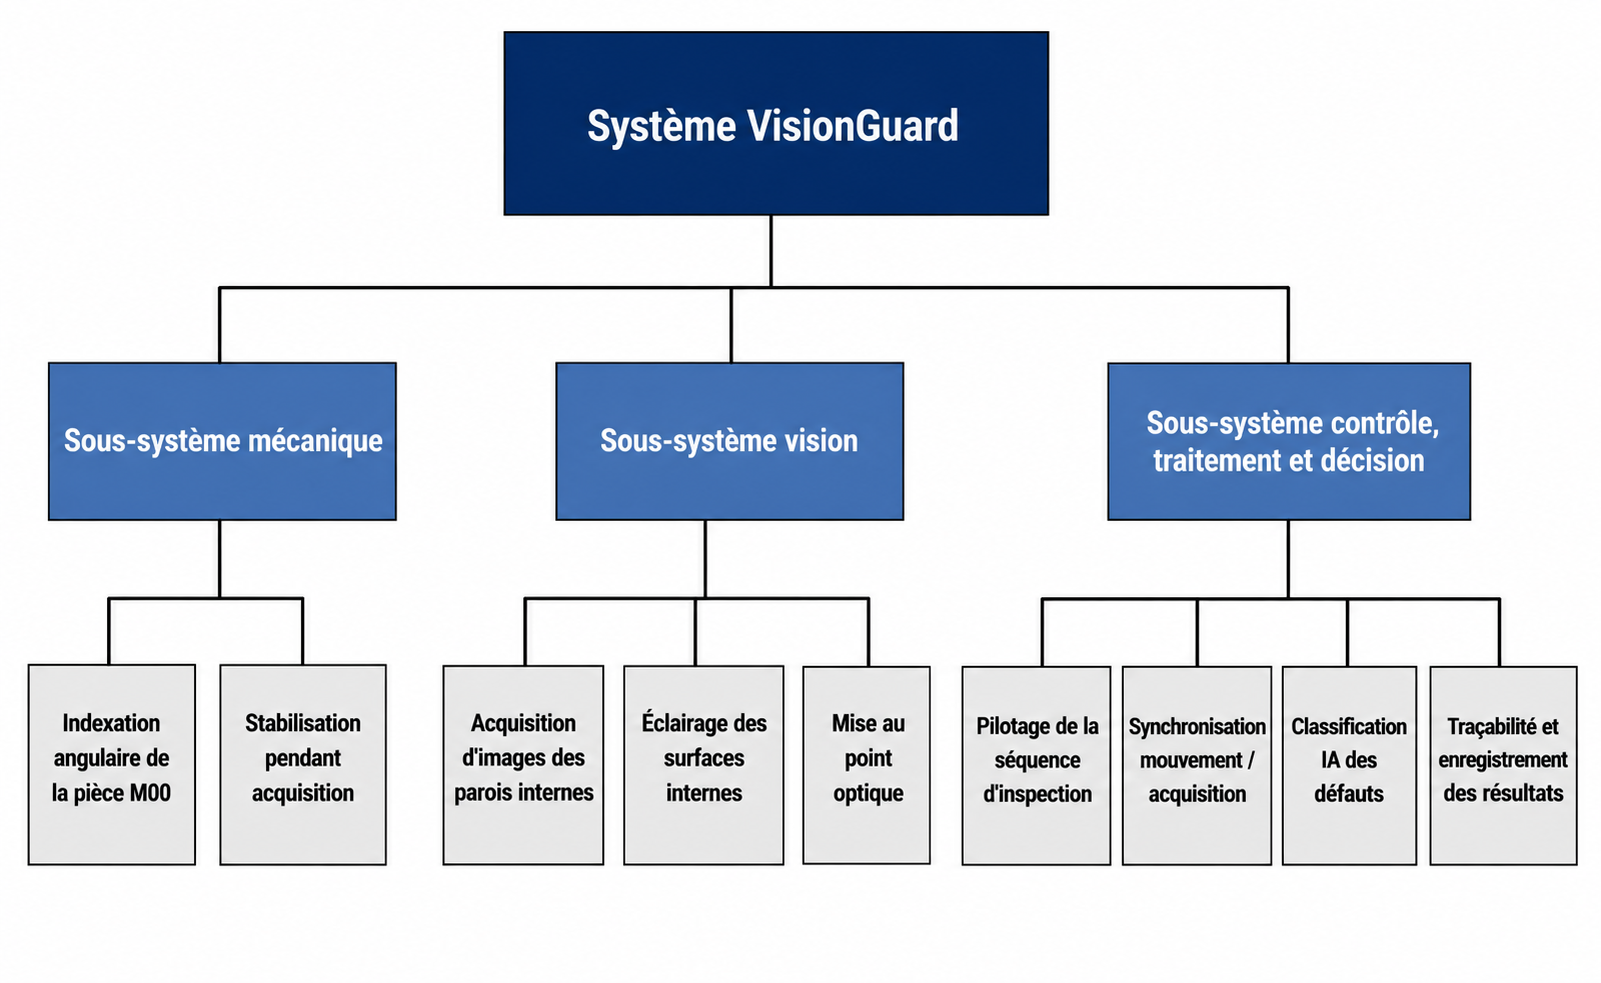
\includegraphics[width=0.95\textwidth]{decomposition_visionguard.png}
    \caption{Schéma de décomposition fonctionnelle du système VisionGuard.}
    \label{fig:decomposition}
\end{figure}

% --------------------------------------------------------
\subsection{Cycle opérationnel d'inspection}

Le cycle opérationnel d'inspection décrit la séquence de fonctionnement du système
VisionGuard depuis le chargement de la pièce jusqu'à l'affichage du résultat final. Ce
cycle se déroule de manière semi-automatisée~: l'opérateur intervient pour préparer et
lancer l'inspection, tandis que la séquence d'acquisition, de traitement et d'enregistrement
est exécutée par le système.

Le cycle nominal se déroule comme suit~:

\begin{enumerate}
    \item L'opérateur place la pièce M00 sur le support rotatif et lance le cycle via
    l'interface utilisateur.
    \item Le système initialise la position de référence et aligne la pièce face à la
    première veine à inspecter.
    \item Le système acquiert une image de la première paroi interne selon l'orientation
    optique définie.
    \item L'orientation optique est ajustée afin d'acquérir l'image de la seconde paroi
    interne de la veine.
    \item Le système indexe la pièce vers la veine suivante selon un pas angulaire
    correspondant à la répartition des veines.
    \item Les étapes d'acquisition et d'indexation sont répétées pour couvrir l'ensemble
    des veines à inspecter.
    \item Les images acquises sont transmises au module de classification par intelligence
    artificielle pour analyse.
    \item Le résultat global PASS/FAIL est affiché à l'opérateur, accompagné de la
    localisation des zones présentant des défauts détectés le cas échéant.
    \item Les images et le résultat sont enregistrés avec horodatage et identifiant pièce
    pour assurer la traçabilité.
\end{enumerate}

\begin{figure}[H]
    \centering
    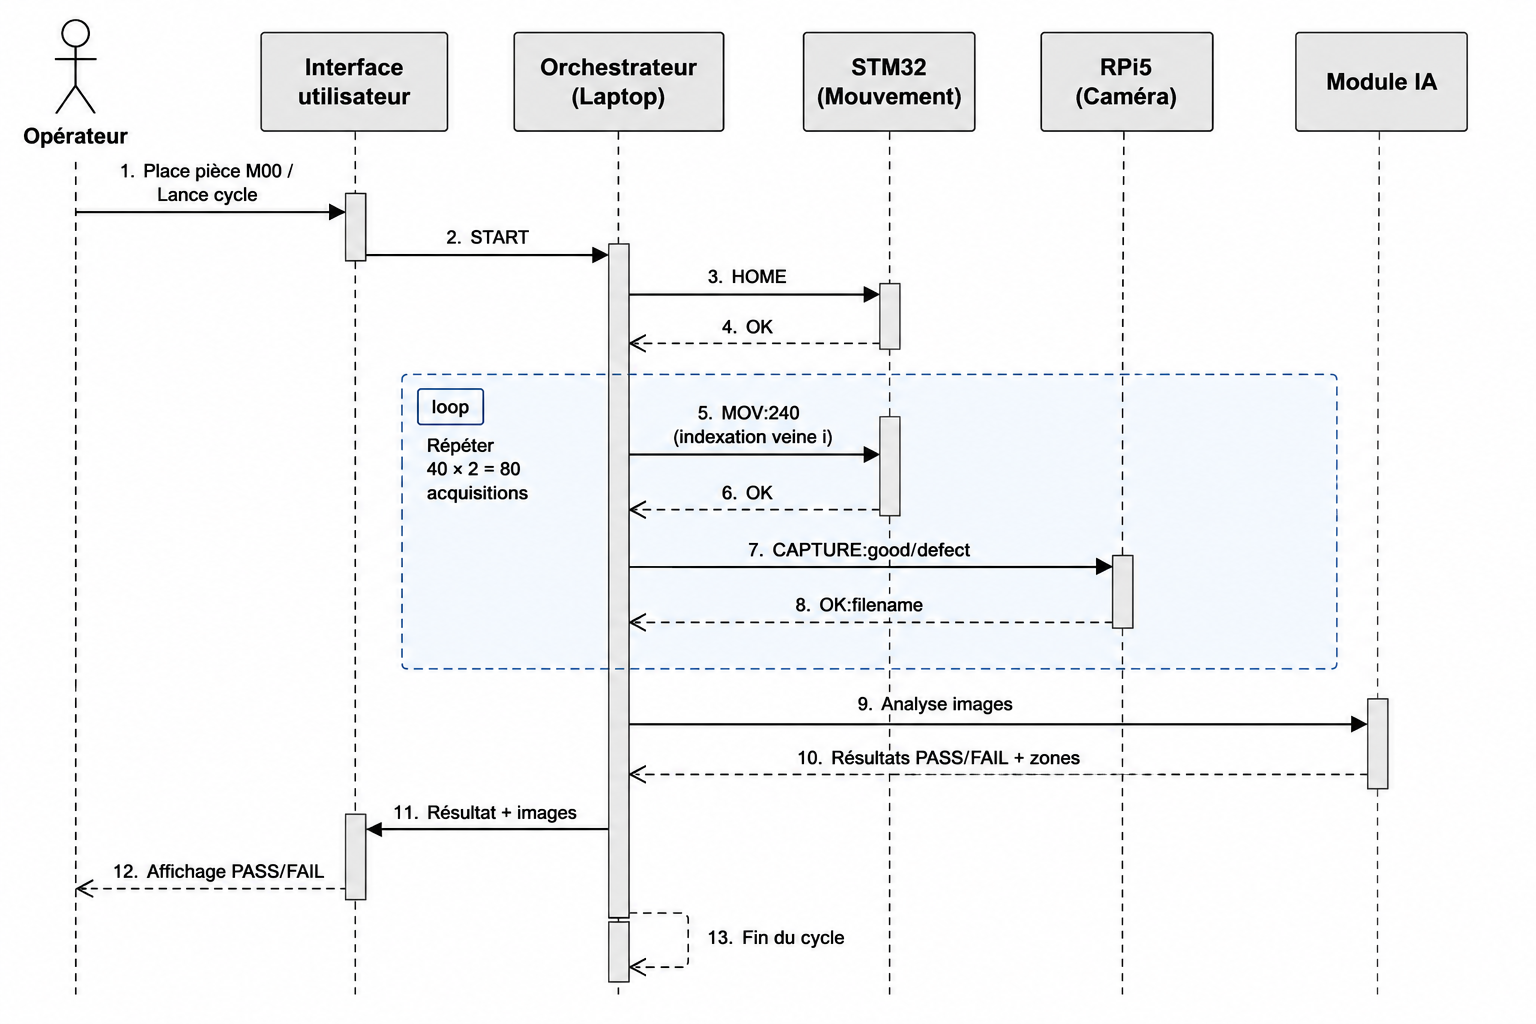
\includegraphics[width=\textwidth]{sequence_visionguard.png}
    \caption{Diagramme de séquence du cycle opérationnel d'inspection.}
    \label{fig:sequence}
\end{figure}

% --------------------------------------------------------
\section{Analyse préliminaire des risques}
% --------------------------------------------------------

L'analyse préliminaire des risques a pour objectif d'identifier les principales défaillances
potentielles du système et de proposer des actions préventives ou correctives avant la phase
de réalisation. Cette analyse s'appuie sur une évaluation de la criticité, de la probabilité
d'occurrence et du niveau de risque résultant.

Le tableau suivant présente une synthèse des risques identifiés lors de la phase de
conception, classés selon leur niveau de criticité.

\renewcommand{\arraystretch}{1.3}
\footnotesize
\begin{longtable}{|p{2.8cm}|p{2.8cm}|c|c|p{1.8cm}|p{7cm}|}
\caption{Analyse préliminaire des risques du système VisionGuard.}
\label{tab:risques} \\
\hline
\rowcolor{gray!20}
\textbf{Risque identifié} & \textbf{Cause probable} &
\textbf{C} & \textbf{P} &
\textbf{Niveau} &
\textbf{Action préventive / corrective} \\
\hline
\endfirsthead
\hline
\rowcolor{gray!20}
\textbf{Risque identifié} & \textbf{Cause probable} &
\textbf{C} & \textbf{P} &
\textbf{Niveau} &
\textbf{Action préventive / corrective} \\
\hline
\endhead
\hline
\endfoot
Images floues ou mal cadrées
    & Vibrations, mauvais réglage optique, profondeur de champ insuffisante
    & 5 & 3 & 15 — Élevé
    & Calibration optique, stabilisation mécanique, pause avant capture \\ \hline
Défaut de positionnement angulaire
    & Jeu mécanique, imprécision d'indexation
    & 4 & 3 & 12 — Moyen
    & Réduction mécanique, vérification des tolérances, tests de répétabilité \\ \hline
Éclairage insuffisant ou non uniforme
    & Positionnement inadéquat des LEDs, puissance trop faible
    & 5 & 4 & 20 — Élevé
    & Tests en conditions réelles, ajustement orientation et intensité \\ \hline
Dataset insuffisant ou déséquilibré
    & Nombre limité de pièces non conformes
    & 5 & 4 & 20 — Élevé
    & Collecte progressive, augmentation des données, validation indépendante \\ \hline
Modèle IA sous-performant
    & Dataset non représentatif, sur-apprentissage
    & 5 & 4 & 20 — Élevé
    & Validation croisée, séparation apprentissage/test, évaluation indépendante \\ \hline
Temps de cycle dépassé
    & Acquisition lente, traitement IA lent
    & 3 & 3 & 9 — Moyen
    & Optimisation séquence, réduction temps morts, parallélisation \\ \hline
Panne composant électronique
    & Défaillance caméra, moteur, driver
    & 4 & 2 & 8 — Faible
    & Documentation câblage, rechanges identifiés, tests unitaires \\ \hline
Accès optique insuffisant
    & Géométrie chevron, angle d'observation limité
    & 5 & 3 & 15 — Élevé
    & Tests optiques préalables, ajustement angle caméra \\ \hline
Vibrations pendant acquisition
    & Rigidité insuffisante, mouvement non stabilisé
    & 3 & 3 & 9 — Moyen
    & Renforcement châssis, pause stabilisation, contrôle fixation caméra \\ \hline
Perte de communication
    & Déconnexion USB/Ethernet, erreur protocole
    & 4 & 3 & 12 — Moyen
    & Protocole simple, accusés de réception, tests séquence complète \\ \hline
\multicolumn{6}{|l|}{\textit{C = Criticité (1--5) \quad P = Probabilité (1--5) \quad Niveau = C $\times$ P \quad Faible~: $\leq$8 \quad Moyen~: 9--12 \quad Élevé~: $\geq$13}} \\
\hline
\end{longtable}
% --------------------------------------------------------
\section{Conclusion}
% --------------------------------------------------------

Ce chapitre a formalisé le besoin industriel selon une approche d'ingénierie système légère.
Le diagramme de contexte a permis de délimiter les frontières du système VisionGuard et
d'identifier les acteurs externes en interaction avec lui. L'analyse des interactions a
structuré les échanges entre le système et son environnement, servant de base à la
spécification des exigences.

Les cas d'utilisation ont décrit les principaux scénarios d'interaction opérationnelle,
tandis que les exigences fonctionnelles et non fonctionnelles ont traduit le besoin en
critères mesurables et vérifiables. Les critères de validation associés établissent le lien
direct entre les exigences définies dans ce chapitre et les essais de validation qui seront
présentés au chapitre~5.

La décomposition fonctionnelle a organisé le système en trois sous-systèmes principaux~:
mécanique, vision, et contrôle-traitement-décision. Le cycle opérationnel d'inspection a
ensuite décrit la séquence générale de fonctionnement, depuis le chargement de la pièce
jusqu'à l'affichage et l'enregistrement du résultat. Enfin, l'analyse préliminaire des
risques a identifié les points critiques nécessitant une attention particulière, notamment
la qualité d'acquisition d'image, la couverture optique des parois internes, la constitution
du dataset et la performance du module IA.

Le chapitre suivant présentera les choix de conception détaillés pour chacun des
sous-systèmes, en justifiant les solutions techniques retenues au regard des exigences
formulées dans ce chapitre.
\chapter{Conception du Système VisionGuard}

\section{Sous-système mécanique}
\subsection{Table d'indexation rotative}
\todo{Décrire la table d'indexation : moteur NEMA17, réduction courroie 3:1, calcul des micropas (240 micropas/veine, 27 micropas/degré à 1/16), précision angulaire.}

\subsection{Mécanisme de positionnement caméra}
\todo{Décrire la rotule ball joint pour la phase PoC, puis le servo DS3218 prévu pour la version complète. Justifier le choix de la démarche progressive.}

\subsection{Structure mécanique}
\todo{Profilés aluminium, supports imprimés 3D, contraintes d'encombrement ($\leq 1$~m²).}

\section{Sous-système de vision}
\subsection{Sélection de la caméra}
\todo{Justifier le choix RPi HQ Camera (IMX296, 1.6 MP, obturateur global, 12-bit ADC) face aux alternatives. Avantage obturateur global pour sujets statiques précis.}

\subsection{Optique}
\todo{Objectif 16 mm C-mount, ouverture f/8--f/11, calcul du champ de vision pour détection $\geq 0.8$~mm.}

\subsection{Éclairage}
\todo{3 LEDs blanches, illumination par le bas des veines. Justifier le choix de l'éclairage bas pour les surfaces internes en céramique matte rose.}

\section{Sous-système électronique et contrôle}
\subsection{Architecture matérielle}
\todo{Décrire les trois nœuds : Laptop (maître), STM32 Nucleo F446RE (contrôle mouvement), RPi5 (acquisition image). Justifier la séparation des rôles.}

\subsection{Driver moteur TMC2208}
\todo{Configuration TMC2208 : Vref = 1.21V (courant RMS $\approx 0.85$A), mode stealthChop, 1/16 microstepping. Justifier le choix par rapport aux alternatives (A4988, DRV8825).}

\subsection{Alimentation}
\todo{Schéma d'alimentation : 220V AC $\rightarrow$ 12V/5A (moteur), 12V $\rightarrow$ 5V (buck converter), 5V/5A USB-C PD (RPi5). Isolation des alimentations.}

\subsection{Assignation des broches STM32}
\begin{table}[H]
\centering
\caption{Assignation des signaux STM32 Nucleo F446RE}
\begin{tabular}{lll}
\toprule
\textbf{Signal} & \textbf{Broche STM32} & \textbf{Connecteur} \\
\midrule
STEP  & PB10 & D6 \\
DIR   & PB5  & D4 \\
UART TX & PA2 & CN10 (USART2) \\
UART RX & PA3 & CN10 (USART2) \\
\bottomrule
\end{tabular}
\end{table}

\section{Sous-système logiciel}
\subsection{Architecture logicielle globale}
\todo{Décrire les trois couches logicielles : firmware STM32 (C/HAL), serveur RPi5 (Python/TCP), orchestrateur Laptop (Python). Schéma des flux de données.}

\placeholderfigure{Flux de données VisionGuard}{Flux de données et séquence de commandes du système VisionGuard}

\subsection{Firmware STM32 — Contrôle mouvement}
\todo{Décrire l'architecture firmware : UART HAL polling, parseur de commandes (HOME/MOV/SPEED), génération STEP/DIR. Justifier HAL polling vs interruptions pour ce cas d'usage.}

\subsection{Serveur RPi5 — Acquisition image}
\todo{Décrire le serveur TCP Python sur RPi5 : écoute commandes CAPTURE/DELETE/QUIT, acquisition picamera2 (1456×1088, XBGR8888), horodatage fichiers, log session JSON.}

\subsection{Orchestrateur Laptop — Coordination système}
\todo{Décrire le script Python maître : envoi commandes UART STM32, envoi commandes TCP RPi5, synchronisation mouvement/capture, interface clavier opérateur.}

\subsection{Protocole de communication UART}
\begin{table}[H]
\centering
\caption{Protocole UART Laptop $\leftrightarrow$ STM32 (115200 baud)}
\begin{tabular}{lll}
\toprule
\textbf{Commande} & \textbf{Description} & \textbf{Réponse} \\
\midrule
\texttt{HOME\textbackslash n}        & Définir position zéro & \texttt{OK\textbackslash n} \\
\texttt{MOV:N\textbackslash n}       & Déplacer N micropas   & \texttt{OK\textbackslash n} \\
\texttt{SPEED:V\textbackslash n}     & Régler vitesse (100--2000 µpas/s) & \texttt{OK\textbackslash n} / \texttt{ERR\textbackslash n} \\
\texttt{READY\textbackslash n}       & Envoyé au démarrage STM32 & — \\
\bottomrule
\end{tabular}
\end{table}

\subsection{Protocole TCP RPi5}
\begin{table}[H]
\centering
\caption{Protocole TCP Laptop $\leftrightarrow$ RPi5}
\begin{tabular}{lll}
\toprule
\textbf{Commande} & \textbf{Description} & \textbf{Réponse} \\
\midrule
\texttt{CAPTURE:good\textbackslash n}   & Capturer image — classe \textit{good}   & \texttt{OK:filename} \\
\texttt{CAPTURE:defect\textbackslash n} & Capturer image — classe \textit{defect} & \texttt{OK:filename} \\
\texttt{DELETE:fname\textbackslash n}   & Supprimer un fichier                    & \texttt{OK} / \texttt{ERR} \\
\texttt{QUIT\textbackslash n}           & Fin de session                          & \texttt{BYE} \\
\bottomrule
\end{tabular}
\end{table}

\section{Module d'intelligence artificielle}
\subsection{Approche de détection}
\todo{Décrire l'approche choisie pour la classification des défauts. Justifier le choix CNN vs approches classiques pour ce type de surface (céramique matte, faible contraste).}

\subsection{Pipeline de collecte de données}
\todo{Décrire la procédure de collecte du dataset : étiquetage \textit{good}/\textit{defect}, commandes clavier, volume cible, visite Pursuit Aerospace.}

\subsection{Architecture du modèle}
\todo{À compléter après entraînement — architecture retenue, hyperparamètres, taille du dataset.}

\section{Conclusion}
\todo{Synthèse de la conception et transition vers le chapitre implémentation/tests.}

\chapter{Implémentation et Tests}

\section{Implémentation matérielle}
\subsection{Assemblage mécanique}
\todo{Décrire l'assemblage : montage moteur, table d'indexation, profilés aluminium, supports 3D. Photos du système assemblé.}

\placeholderfigure{Système assemblé VisionGuard}{Système VisionGuard assemblé — vue d'ensemble}

\subsection{Câblage électronique}
\todo{Décrire le câblage complet : PSU, TMC2208, STM32, RPi5, LEDs éclairage. Schéma de câblage.}

\placeholderfigure{Schéma câblage}{Schéma de câblage électronique du système VisionGuard}

\section{Implémentation logicielle}
\subsection{Environnement de développement}
\todo{Ubuntu 22.04, VS Code, pyenv Python 3.11.9, STM32CubeIDE 2.1.1, dépendances Python.}

\subsection{Firmware STM32}
\todo{Décrire l'implémentation firmware : configuration CubeMX, timer STEP, UART HAL polling, tests unitaires réalisés.}

\subsection{Scripts Python}
\todo{Décrire l'implémentation des scripts : rpi5\_server.py, collect\_orchestrator.py, structure du dépôt GitHub.}

\section{Tests et validation}
\subsection{Tests du sous-système mécanique}
\todo{Tests d'indexation : précision angulaire mesurée, répétabilité, vitesse. Résultats numériques.}

\subsection{Tests du sous-système vision}
\todo{Tests optiques : résolution effective sur pièce M00, détection visuelle de défauts $\geq 0.8$~mm, conditions d'éclairage.}

\subsection{Tests d'intégration système}
\todo{Tests de la chaîne complète : motion + capture + transfert. Mesure du temps de cycle par veine.}

\subsection{Entraînement et validation du modèle IA}
\todo{Décrire le dataset collecté (volume, répartition classes), l'entraînement, les métriques obtenues (précision, rappel, F1-score, matrice de confusion).}

\section{Conclusion}
\todo{Synthèse des résultats de tests et transition vers le chapitre résultats/validation.}

\chapter{Résultats et Validation}

\section{Résultats du système d'inspection}
\subsection{Performance du sous-système mécanique}
\todo{Tableaux de mesures : précision angulaire, répétabilité, temps d'indexation par veine.}

\subsection{Performance du sous-système vision}
\todo{Résolution spatiale effective, qualité d'image sur M00, sensibilité détection 0.8 mm.}

\subsection{Performance du modèle IA}
\todo{Métriques finales : précision, rappel, F1-score, AUC. Matrice de confusion. Exemples d'images correctement et incorrectement classifiées.}

\subsection{Performance globale — temps de cycle}
\todo{Mesure du temps de cycle complet par pièce M00 (40 veines, 80 surfaces). Comparaison avec l'objectif $\leq 3$~min.}

\section{Validation des critères de succès}
\begin{table}[H]
\centering
\caption{Validation des critères de succès VisionGuard}
\begin{tabular}{lll}
\toprule
\textbf{Critère} & \textbf{Objectif} & \textbf{Résultat} \\
\midrule
Détection défauts $\geq 0.8$~mm  & 100\% détection  & \todo{à mesurer} \\
Temps de cycle                    & $\leq 3$~min/pièce & \todo{à mesurer} \\
Précision modèle IA               & $> 90\%$         & \todo{à mesurer} \\
Rappel modèle IA                  & $> 90\%$         & \todo{à mesurer} \\
Reproductibilité                  & Résultats stables & \todo{à évaluer} \\
\bottomrule
\end{tabular}
\end{table}

\section{Discussion}
\todo{Analyser les résultats obtenus face aux objectifs. Identifier les limites du système PoC. Proposer des pistes d'amélioration pour une version industrielle.}

\section{Perspectives d'industrialisation}
\todo{Décrire le chemin vers une version industrielle : intégration servo DS3218, robustesse, interface HMI, traçabilité, intégration au flux de production Pursuit.}

\section{Conclusion}
\todo{Synthèse des résultats et transition vers la conclusion générale.}

\chapter*{Conclusion Générale}
\addcontentsline{toc}{chapter}{Conclusion Générale}

\todo{Rédiger la conclusion générale ici. 1--1.5 pages. Rappel de la problématique, synthèse des contributions (mécanique, vision, contrôle, IA), résultats obtenus, limites, perspectives à court et long terme.}


% =========================
% Annexes
% =========================
\appendix
\chapter{Schémas Électroniques et Câblage}

\section{Schéma de câblage complet}
\placeholderfigure{Schéma câblage complet}{Schéma de câblage complet du système VisionGuard}

\section{Configuration TMC2208}
\todo{Tableau des paramètres TMC2208 : Vref, courant, microstepping, mode stealthChop.}

\chapter{Extraits de Code Source}

\section{Firmware STM32 — Parseur de commandes UART}
\todo{Insérer ici l'extrait de code firmware STM32 du parseur UART.}

\begin{lstlisting}[language=C, caption={Parseur de commandes UART — STM32 HAL}]
% TODO: inserer extrait firmware ici
\end{lstlisting}

\section{Script RPi5 — Serveur TCP acquisition}
\todo{Insérer ici l'extrait principal du rpi5\_server.py.}

\begin{lstlisting}[language=Python, caption={Serveur TCP RPi5 — acquisition image}]
%TODO: inserer extrait rpi5_server.py ici
\end{lstlisting}


% =========================
% Bibliographie
% =========================
\printbibliography[heading=bibintoc,title={Bibliographie}]

\end{document}
